\section{Jet b tagging}\label{sec:btag}

Jets that arise from bottom quark hadronization (b-jets) are present in many physics processes,
such as the decay of top quarks. The ability to accurately identify b-jets is crucial to reduce the otherwise overwhelming background from these processes to channels involving jets from gluons (g) and
light-flavour quarks (u, d, s), and from c-quark fragmentation.

Algorithms for b jet identification (also known as b tagging algorithms) exploit the long life time of b hadrons present in jets originating from the hadronization of b quarks. This long life time results in a decay of the b hadron that is displaced with respect to the primary interaction vertex. This displacement of a few millimetres results in the presence of displaced tracks from which a secondary vertex may be reconstructed. In addition, b hadrons have a probability of around 20\% to decay to a muon or electron. Hence, also the presence of these charged leptons can be exploited for b jet identification techniques and for measuring their performance with the collision data.

A variety of reconstructed physics objects, as tracks, vertices and identified leptons, can be used to build observables that discriminate between b and light-quark jets. Several b tagging algorithms have been developed by CMS, each one based on different input information. A common feature of all the algorithms is that each one yields a single discriminator value for each jet, which measures the likelihood that the jet has been produced by the hadronization of a b quark. The minimum thresholds on these discriminators define loose (``L''), medium (``M''), and tight (``T'') operating points with a misidentification probability for light-parton jets close to 10\%, 1\%, and 0.1\%, respectively, at an average jet \pt of about 80\,\GeV. The misidentification probability, also known as mistag rate, is defined as the probability to wrongly identify a light-parton jet as a b-jet.

Some of the algorithms make use of the track impact parameters (IP) with respect to the primary vertex, defined as the distance between the primary vertex and the track at their point of closest approach, to distinguish the decay products of a b hadron from prompt tracks. The impact parameter has the same sign as the scalar product of the vector pointing from the primary vertex to the point of closest approach with the jet direction. Tracks originating from the decay of particles travelling along the jet axis will tend to have positive IP values. In contrast, the impact parameters of prompt tracks can have positive or negative IP values. The impact parameter significance, defined as the ratio of the IP to its estimated uncertainty, is used as an observable.

The \emph{Track Counting} (TC) algorithm sorts tracks inside a jet by decreasing values of the IP significance. Although the ranking tends to bias the values for the first track to high positive IP significances, the probability to have several tracks with high positive values is low for light-parton jets. Therefore the two different versions of the algorithm use the IP significance of the second and third ranked track as the discriminator value.  These two versions of the algorithm are called \emph{Track Counting High Efficiency} (TCHE) and \emph{Track Counting High Purity} (TCHP), respectively.

A general extension of the TC algorithm, i.e. the \emph{Jet Probability} (JP), combines the IP information of several tracks inside the jet, using an estimate of the likelihood that all tracks associated to the jet come from the primary vertex as a discriminating variable. A variant of
the JP algorithm also exists in which the four tracks with the highest impact parameter significance get a higher weight in the jet probability calculation. This algorithm is referred to as \emph{Jet B-Probability} (JBP).

A different approach consists in using the secondary vertices and the related kinematic variables, together with displaced tracks information, to discriminate between b and non-b jets. This algorithm is known as \emph{Combined Secondary Vertex} (CSV)\footnote{An improved version of this algorithm, CSVv2, has been developed for Run 2 analyses.}. The magnitude and direction of the vector connecting the primary and secondary vertices are used as a discriminating variables and quality requirements are imposed to secondary vertex candidates. In addition, the usage of displaced tracks information allows to increase the efficiency for events where no secondary vertex is found. Several variables related to secondary vertices and displaced tracks are used to build likelihood ratios that have a good discriminating power.

Two algorithms for reconstructing secondary vertices are exploited. For the first algorithm, the
tracks associated to jets and fulfilling some quality requirements are used in the adaptive vertex reconstruction (AVR) algorithm~\cite{Waltenberger:1166320}. The AVR is the algorithm used for CMS analyses during the 8\,\TeV data taking. In contrast with this method, the Inclusive Vertex Finder (IVF) algorithm is not seeded from tracks associated to reconstructed jets, but instead makes use of all the tracks in the event, with appropriate selections, to reconstruct the secondary vertices. The latter is the default algorithm used to reconstruct secondary vertices for CMS analyses using 13\,\TeV data.

A new b jet identification algorithm has been recently developed, combining the discriminators provided by the JP and CSV algorithms with a Boosted Decision Tree (BDT) technique. This combined multivariate algorithm (cMVA) is found to slightly improve the b jet identification efficiency.

The performance of these algorithms is determined using simulated \ttbar events, selecting events with at least one jet with $\pt > 30$\,\GeV. This is shown in Fig.~\ref{fig:btagperf}, where the b jet identification efficiency versus the misidentification probability is reported for the various algorithms. This figure serves as an illustration as the b tagging performance depend on the \pt and $\eta$ distribution of the jets, and need to be checked for each analysis phase space.

\begin{figure}[htb]
\centering
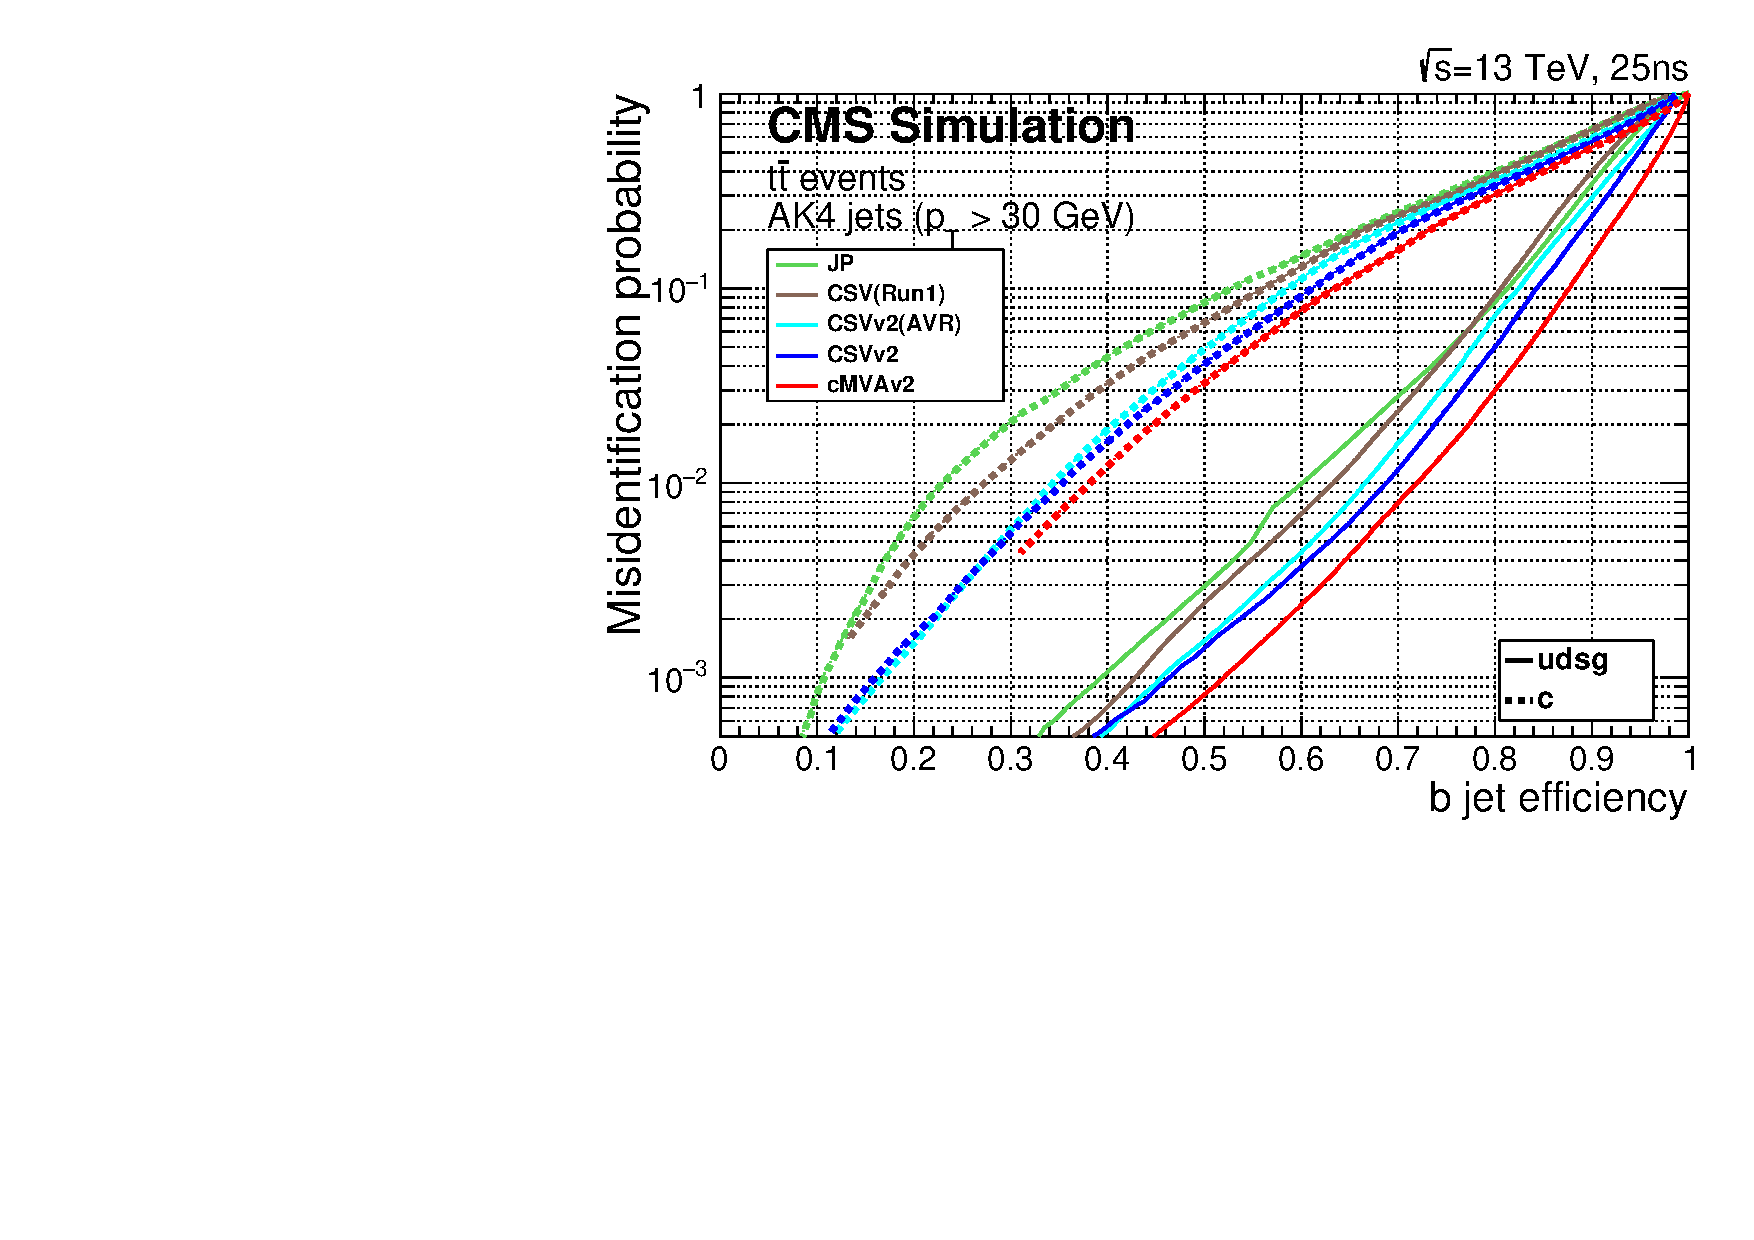
\includegraphics[width=0.7\textwidth]{images/btagperf.pdf}
\caption{Performance of the b jet identification efficiency algorithms demonstrating the probability for non-b jets to be misidentified as b jet as a function of the efficiency to correctly identify b jets. The curves are obtained on simulated \ttbar events using anti-$k_t$ jets clustered with $R=0.4$ and requiring $\pt>30$\,\GeV.}\label{fig:btagperf}
\end{figure}


